\section{模型接入}

凡是逐行读文字的节点，都要一个模型。模型有两个来源，二选一。

\begin{figure}[H]\centering
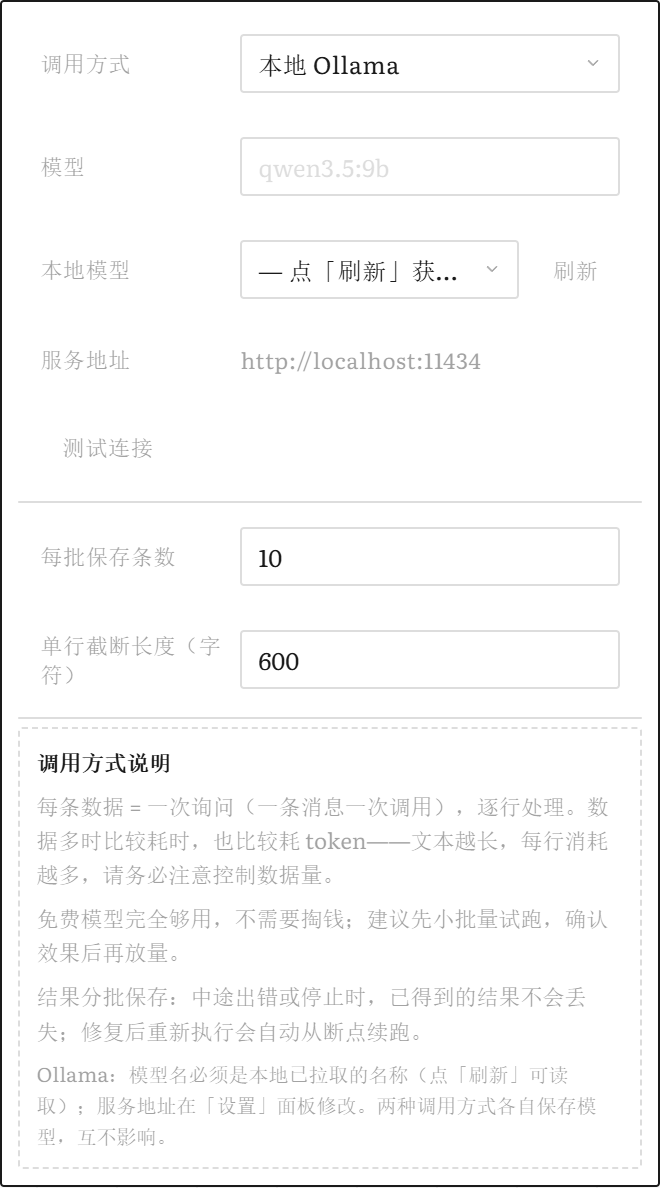
\includegraphics[width=0.58\textwidth]{ai-menu.png}
\caption{顶栏的模型菜单：提供方、模型、本地模型、服务地址、批量}
\label{fig:ai-menu}
\end{figure}

\subsection{本地 Ollama}

本机装 Ollama，拉一个模型，比如 \texttt{qwen3.5:9b}。菜单里调用方式选本地 Ollama，服务地址默认 \texttt{http://localhost:11434}。
点“\texttt{刷新}”读本机已有的模型列表，点“\texttt{测试连接}”看通不通。本地模型的优点是不要钱、不联网、数据不出机器；
缺点是吃显存与内存，长文本要截断。

\subsection{OpenRouter}

不想在本机跑大模型时用 OpenRouter。Key 只存在浏览器里，不写到服务器，也不进数据库，换一台机器要重新填一次。

\subsection{两个层级}

菜单里选的是这一整轮运行的默认模型。每个用本地模型的分析节点还可以在自己面板里单独挑一个，默认跟随全局。
这样一条链里可以让清洗用小模型，主题概括用大模型。

\subsection{批量与截断}

两个数字管成本。每批保存条数决定多久落一次盘，太小会慢，太大中断时损失多；单行截断长度决定一条文本最多送多少字，超出部分截掉。
逐行调用的结果都按提示词缓存，同一张表重跑，已经问过的行不再花钱。中途停下，没处理的行留成未处理，节点算部分完成，不会被标成成功。

\section{情感分析的三条路}

情感这一件事有三种做法，面板上一个下拉切换。选哪种，取决于你有多少数据、要不要理由、机器扛不扛得住。

\begin{figure}[H]\centering
\begin{tikzpicture}
  \node[card=src,text width=3.4cm] (start) at (0,0) {要分析一列文本};
  \node[chip,text width=3.4cm] (llm) at (-4.6,-1.9) {大模型\\[1pt]逐行读，给理由};
  \node[chip,text width=3.4cm] (ml) at (0,-1.9) {传统机器学习\\[1pt]本地拟合，批量快};
  \node[chip,text width=3.4cm] (bert) at (4.6,-1.9) {微调 BERT\\[1pt]默认推荐};
  \draw[softwire] (start.south) -- (llm.north);
  \draw[softwire] (start.south) -- (ml.north);
  \draw[softwire] (start.south) -- (bert.north);
  \node[chip,below=10mm of bert,text width=3.4cm,draw=errc!60] (fallback) {跑不动时降到机器学习\\[1pt]并打印实际用的模式};
  \draw[wire] (bert) -- (fallback);
  \node[micro,below=3mm of ml] {几万行首选};
  \node[micro,below=3mm of llm] {几百行以内};
\end{tikzpicture}
\caption{三条路与一条降级路径}
\label{fig:sentiment-modes}
\end{figure}

\begin{figure}[H]\centering

\includegraphics[width=0.31\textwidth]{panel-process.png}
\caption{处理节点：操作、文本列、分析模式与模型参数}
\label{fig:panel-process}
\end{figure}

\subsection{传统机器学习}

本地拟合，不吃显卡，一次跑几万行也很快，适合先摸个底看整体倾向。训练基于已标注的行，标注质量决定上限。
面板里的“\texttt{训练 ML 模型}”就是拿当前表里已经标好的行现学一遍。

\subsection{微调 BERT}

默认推荐。它是中文预训练模型在本领域语料上微调过的版本，判断稳、速度快、结果可重复。面板里选一个已注册的模型即可，
勾多个会做多模型对比。跑不动时，比如缺运行环境或者找不到模型，执行器自动降级到机器学习，并在控制台打印这一轮实际用的是哪种。
它不会把降级结果说成 BERT，这一点在写论文时很重要。

\subsection{大模型}

适合样本不大、需要理由的场合。它逐行读，能给出判断与解释，慢，也花 token。提示词固定，所以同一个输入永远得到同一个输出，结果可复现。

\subsection{阈值在哪}

情感极性这一路输出两列：三分类标签与零到一的分数。分数落在两个阈值之间算中性，默认正面下限 0.6、负面上限 0.4，
两个都能在面板里调。阈值是参数不是常数，因为不同语料的分数分布不一样。

\section{多模型对比}

同一列文本，可以让几个模型各判一遍，看它们分歧在哪。在情感、情绪、倾向三个节点的面板里勾两个以上已注册的模型，
执行时每个模型各跑一遍，输出一张长表：原表每一行乘每个模型一行，另加一列模型名和一列原行号，方便把同一个句子的几个判断对起来。
只勾一个模型时不拉长表，就在原表上加列，老画布不受影响。

分歧本身是信息。两个模型都判负面基本可以信；一个判正面一个判负面，那几行值得人看一眼，往往正是反讽、引用、转述这类机器容易错的地方。

图上有两种看法：模型乘标签的分布用热力图，一眼看出哪个模型偏乐观；模型之间的一致率用专门的图，按两两模型判定相同的百分比画方阵。
列不全或者模型不足两个时会拒绝，不画一张一格的空图。多模型对比不降级：选了两个模型却跑不动，按名字拒绝，不会悄悄只跑一个然后说跑完了。

模型注册表是一个 JSON 文件，登记模型的名字、路径、属于哪个操作，面板上就出现可勾选的名字，换机器也不会因为路径写死而失效。
文件缺失时复选框整组消失，手动填路径的框还在。

\section{其他分析算子}

情感之外还有一批常用分析，都在分析节点的操作下拉里。

\begin{itemize}
\item 关键词提取。TF-IDF 与 TextRank 两档，还可以只按自己语料算权重，避免新闻语料的词频干扰。
\item 文本聚类。K-Means 与 DBSCAN；K-Means 要指定簇数，DBSCAN 按密度自己找，还会标出噪声点。
\item 命名实体识别。规则模式零依赖，模型模式更全，可以只留人名、地名、机构、日期里的某几类。
\item 异常检测。孤立森林标数值异常行；少于五行或者没有数值列时直接报错，不给每行填零分。
\item 相关性分析。Pearson、Spearman、Kendall 三种系数，选文本列会报错并点名。
\item 显著性检验。一个类别列分组，一个数值列取值，四种方法覆盖参数与非参数，p 值取真实分布。
\item 水军可能性。按作者读整表，看文本雷同程度与发帖突发度，给出线索分，不是判决。
\item 网暴言论识别。按谩骂、人身攻击、隐私披露、造谣转述四类特征打分，默认词库模式。
\item 聚类摘要与簇综述。请模型给每个簇写一段话，前者读簇内文本，后者读簇的度量。
\end{itemize}

网暴识别多说一句。词库模式明说自己是召回器不是判定器，换个说法的攻击看不见，这个不足写不进结果表，所以词表放在代码里让它可以被检查。
隐私披露权重高于谩骂，辟谣用词故意不算暴力。要覆盖委婉语与谐音，切到模型模式。

\section{主题模型}

主题模型回答一个问题：这一堆文本在谈几件事，每件事用什么词。

默认方法“\texttt{自动}”：装了句向量模型就用句向量加聚类，没装就用 LDA。两条路都会在控制台写明这一次实际走了哪条，
绝不把自动降级说成向量。想固定一种就在方法里明说；选向量但环境里没有编码器，节点按名字拒绝，不偷偷换成 LDA。
困惑度是 LDA 自己的量，走向量时这个字段留空，不伪造一个看起来能比的数。

不知道填几个主题时，先用“\texttt{主题数扫描}”：它对二到八个主题各拟合一次，给出困惑度与一致性，输出一张表。
看一致性最高的那一段，再结合主题好不好解释，定一个数。真实项目常常分阶段各定一个数，刘学州那条工作流用的是五、六、七、六、三，
每个阶段按自己的语料单独扫描。

“\texttt{分阶段 LDA}”先按阶段列把语料切开，每个阶段单独建模，输出阶段、主题编号、特征词、权重、该主题的帖子数、困惑度、代表文本。
每阶段主题数可以填一个总数，也可以逐段列举。它还会补一列阶段序号，原因上一章讲过，只有数字能跨过节点边界。

“\texttt{主题概括}”每个主题问一次模型，写一句不超过十五字的话。默认任何一个主题失败就让节点失败，也可以切成留空继续。
没配模型时开始前就拒绝，不会先花钱再报错。答案按提示词缓存，同一张表重跑不再付费。

\section{主题的四张图}

主题分析产出的是表，图在下一步。四张图对应四种看法。

\begin{figure}[H]\centering
\begin{tikzpicture}[node distance=6mm,scale=0.95,transform shape]
  \node[card=src,text width=2.6cm] (stage) {阶段语料};
  \node[card=anl,right=of stage,text width=2.6cm] (lda) {分阶段主题};
  \node[chip,right=of lda,text width=2.7cm] (map) {距离图\\[1pt]主题之间的远近};
  \node[chip,above right=2mm and 5mm of map,text width=2.7cm] (terms) {显著词图\\[1pt]主题自己的词};
  \node[chip,below right=2mm and 5mm of map,text width=2.7cm] (flowg) {桑基图\\[1pt]主题怎么迁移};
  \node[chip,below=6mm of lda,text width=2.7cm] (life) {生命周期\\[1pt]哪些主题跨阶段存活};
  \draw[wire] (stage) -- (lda);
  \draw[wire] (lda) -- (map);
  \draw[softwire] (map) -- (terms);
  \draw[softwire] (map) -- (flowg);
  \draw[softwire] (lda) -- (life);
\end{tikzpicture}
\caption{从阶段语料到四张图}
\label{fig:topic-flow}
\end{figure}

“\texttt{主题距离图}”一行一个主题，给坐标、主题占比、文档数、特征词。坐标由主题之间词分布的散度降维得到，符号固定，
所以同一张表每次画出来一样；气泡大小绑主题占比，一眼看出谁是大主题。

“\texttt{显著词图}”一行一个主题和词，同时给全库频次与主题内频次，两根柱子并排，谁在这个主题里格外突出就看出来了。
排序用相关性，参数 lambda 决定偏向主题内还是偏向全库的溢出，默认零点五，两端都试一次很正常。

“\texttt{主题生命周期}”按特征词的重合度把同一个主题跨阶段追下去，输出首现、峰值、末现、覆盖几个阶段、以及是不是次生。
次生的判据有两条：不是开场那个主题，并且峰值出现在首现之后。这两个条件是论文里的定义，程序照着实现。

“\texttt{主题流向}”对相邻两个阶段的主题两两算相似度，超过阈值的连一条边，正好是桑基图的输入。
一条边都达不到阈值时它拒绝，并告诉你实测最相似的一对是多少，不画一张空桑基。

\begin{figure}[H]\centering
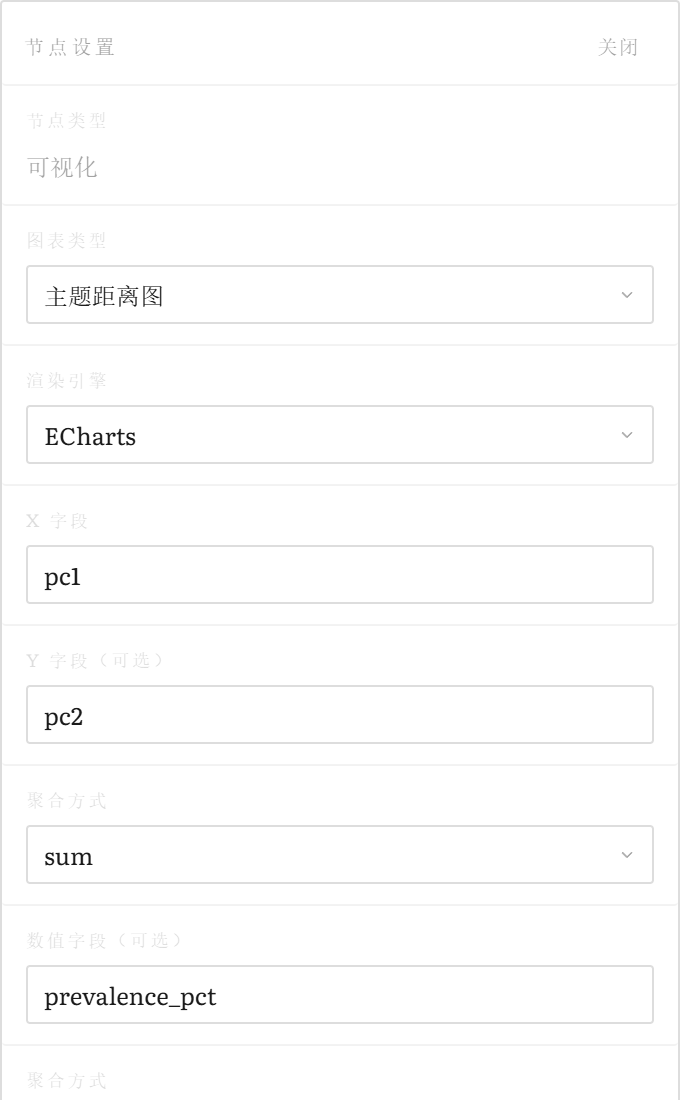
\includegraphics[width=0.31\textwidth]{liu-topicmap.png}
\caption{主题距离图的参数：坐标、标签、气泡大小三列都要指定}
\label{fig:liu-topicmap}
\end{figure}

\section{情感演化与预警}

把情感按阶段或按天算成一个指标，再往后推几期，就得到一条可以讲故事的曲线。

“\texttt{情感演化曲线}”输入一列标签一列分数，输出积极、中性、消极的数量与占比，外加一个情感指数。
指数是积极减消极再除以总数，落在负一到一之间；还可以加一列情感强度，由分数与中点的距离换算，衡量情绪有多激烈。
面板里要指定标签列的三种取值，不同模型给的词不一样，有的是 positive 与 negative，有的是中文，所以这一步不能猜，必须写成实际的值。

分组列选日期得到每日曲线，选阶段得到阶段之间的对比，两个都跑一遍很常见：一张看形状，一张看结论。
有阶段序号时把序号列也填上，否则中文阶段名会被排错。

\begin{figure}[H]\centering
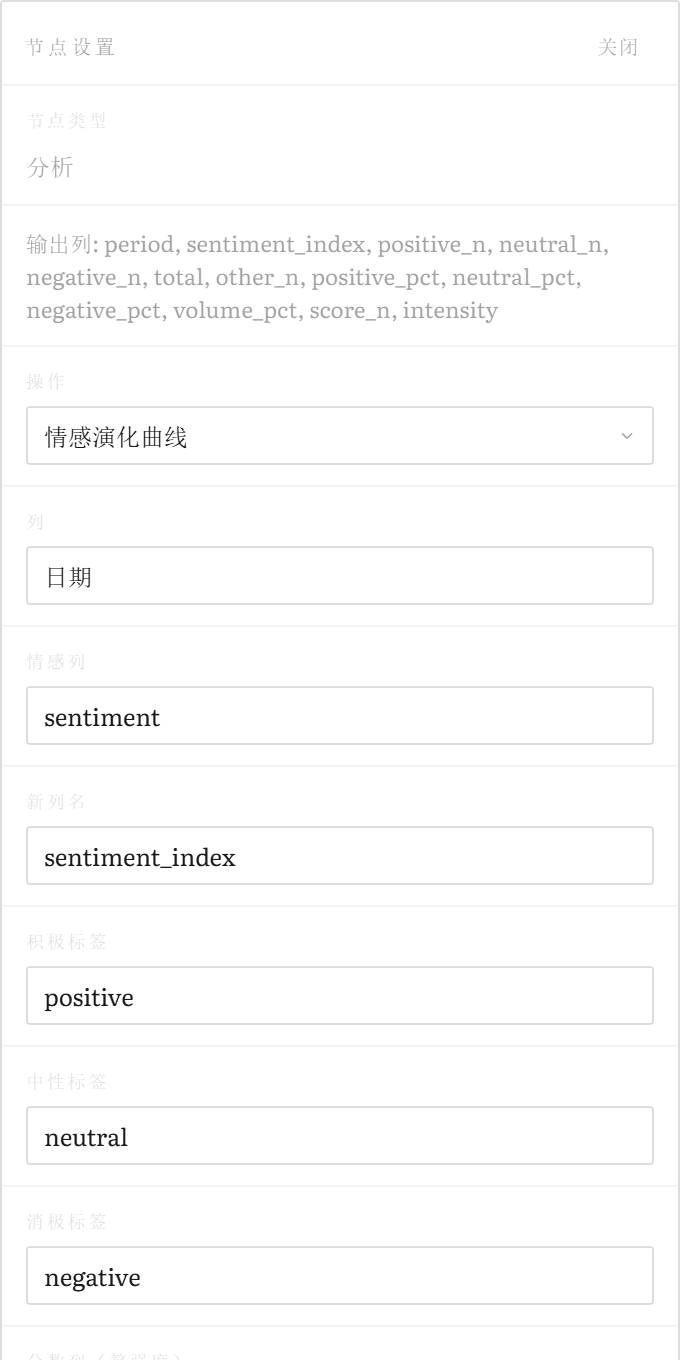
\includegraphics[width=0.31\textwidth]{liu-evolution.png}
\caption{情感演化节点：标签、分数、分组、序号四组参数}
\label{fig:liu-evolution}
\end{figure}

“\texttt{情感走向外推}”把曲线往后推若干期，两种方法，移动平均与 Holt 指数平滑，都是手算，不依赖额外库。
时段列必须能解析成日期，“发酵期”这种名字没法外推，直接拒绝。它推的是曲线的形状，不是预言。

“\texttt{二次爆发预警}”把人的判断写成一条规则。转向是连续若干期同向超过阈值，升温是情感强度每一步都在涨，
两个条件都要求热度还在。一条都没触发时也会给一行未触发，并带上实测到的最大幅度。

\begin{figure}[H]\centering
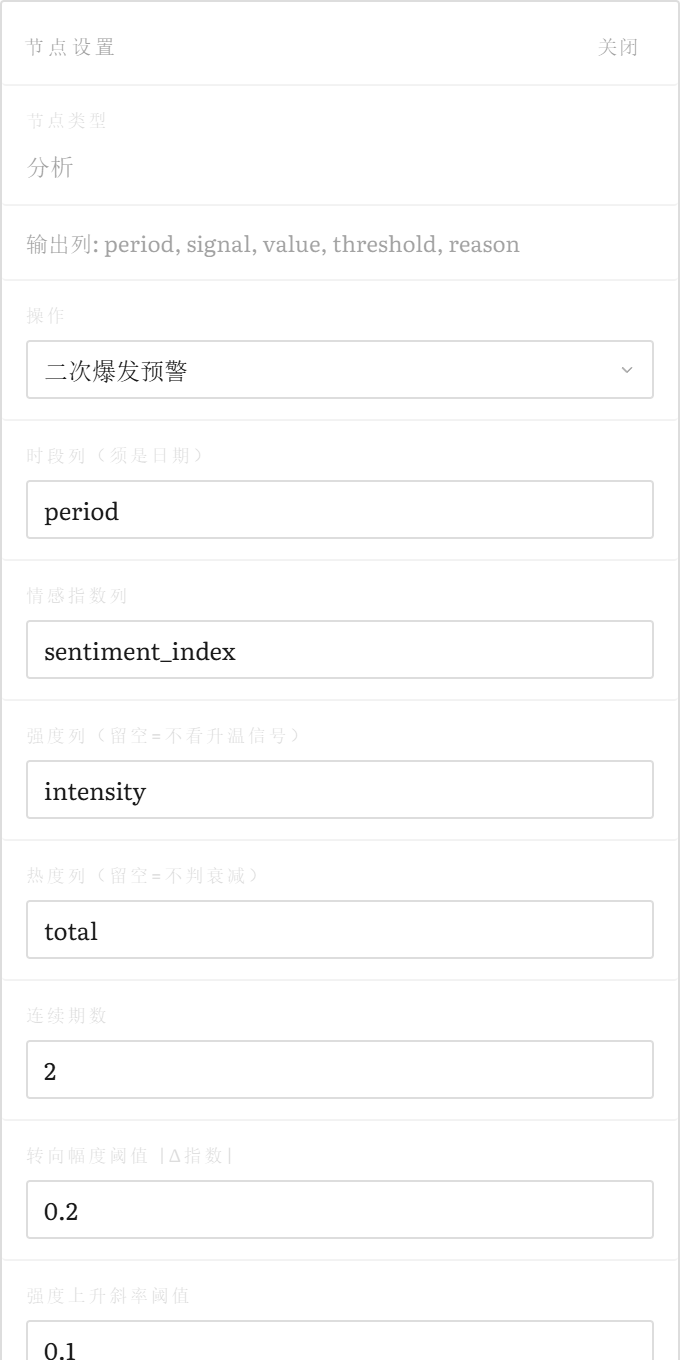
\includegraphics[width=0.31\textwidth]{liu-alert.png}
\caption{二次爆发预警：阈值、连续期数、热度下限}
\label{fig:liu-alert}
\end{figure}

刘学州那次运行里，预警在二月二十二日捕捉到一次转向加升温，强度斜率超过阈值，但当期声量只有三条，
低于前两期均量的六成，所以标成已抑制。四天以后声量配合上来，二次爆发才真正成形。
预警看的是两件事：情绪先行，声量确认。
